\documentclass[11pt]{article}
\usepackage{amsfonts} 

\usepackage{graphicx}%Вставка картинок правильная

\usepackage{float}%"Плавающие" картинки

\usepackage{wrapfig}%


\begin{document}

{\centering
  \large Solution for Home Assignment 1 (Theoretical part)\\
   Danis Alukaev BS19-02\\ \par
}

\bigbreak
\noindent $\textbf{3.1. Big O Notation}$.\\

\noindent \textbf{1.Prove or disprove} that $T(n)=\frac{n^{2}}{3}-3n$ is $O(n^{2})$.\\
By definition of O-Notation, we have to to prove that \\$\exists c, n_{0} > 0$ such that $0 \leq \frac{n^{2}}{3}-3n \leq cn^{2}$ for all $n \geq n_{0}$. \\
Let us divide both sides by $n^{2}\geq0$, then we have $0 \leq \frac{1}{3}-\frac{3}{n} \leq c$.\\
This inequality is satisfied by $c=\frac{1}{3}$ and $n_{0}=9$.\\
Hence, $\frac{n^{2}}{3}-3n=O(n^{2})$ by definition of Big-O.\\
\noindent \textbf{2.Prove or disprove} that $T(n)=k_{1}n^{2}+k_{2}n+k_{3}$ is $O(n^{2})$\\
By definition of O-Notation, we have to to prove that \\$\exists c, n_{0} > 0$ such that $0 \leq k_{1}n^{2}+k_{2}n+k_{3} \leq cn^{2}$ for all $n \geq n_{0}$.
\\
First approach.\\
One can notice that $k_{1}n^{2} \leq k_{1}n^{2}$, $k_{2}n \leq k_{2}n^{2}$ and $k_{3} \leq k_{3}n^{2}$ for all $n \geq 1$. It means that $k_{1}n^{2}+k_{2}n+k_{3} \leq k_{1}n^{2}+k_{2}n^{2}+k_{3}n^{2}$ that is exactly $n^{2}(k_{1}+k_{2}+k_{3})$.\\
Therefore, $k_{1}n^{2}+k_{2}n+k_{3} \leq n^{2}(k_{1}+k_{2}+k_{3})$, $c=k_{1}+k_{2}+k_{3}$ and $n_{0} \geq 1$\\ 
Second approach.\\
Let us divide both sides by $n^{2}\geq0$, then we have $0 \leq k_{1}+\frac{k_{2}}{n}+\frac{k_{3}}{n^{2}} \leq c$.\\
This inequality is satisfied by $c=k_{1}+k_{2}+k_{3}$ and $n_{0}=1$.\\
Hence, $k_{1}n^{2}+k_{2}n+k_{3}=O(n^{2})$ by definition of Big-O.\\
\noindent \textbf{3.Prove or disprove} that $T(n)=3^{n}$ is $O(2^{n})$.\\
By definition of O-Notation, we have to to prove that \\$\exists c, n_{0} > 0$ such that $0 \leq 3^{n} \leq c2^{n}$ for all $n \geq n_{0}$. \\
So, we need to solve such inequality $3^{n} \leq c2^{n}$ to find $c$.\\
Let us divide both sides by $2^{n}\geq0$, then we have $\frac{3}{2}^{n} \leq c$.\\
$\frac{3}{2}^{n}$ is continuous and unbounded function, so there is no such a constant $c$ to satisfy this inequality.\\
Hence, $3^{n}\neq O(2^{n})$ by definition of Big-O.\\
\noindent \textbf{4.Prove or disprove} that $T(n)=0.001 n log(n) - 2000 n + 6$ is $O(n log(n))$\\
By definition of O-Notation, we have to to prove that \\$\exists c, n_{0} > 0$ such that $0.001 n log(n) - 2000 n + 6 \leq cn log(n)$ for all $n \geq n_{0}$.\\ 
One can notice that $0.001 n log(n) \leq 0.001 n log(n)$, $-2000n \leq n log(n)$ and $6 \leq 6 n log(n)$ for all $n\geq2$. It means that $0.001 n log(n) - 2000 n + 6 \leq 0.001 n log(n) + n log(n) + 6 n log(n)$ that is exactly $7.001n log(n)$.\\
So, mentioned inequality is satisfied by $c=7.001$ and $n_{0}=2$.\\
Hence, $0.001 n log(n) - 2000 n + 6=O(n log(n))$ by definition of Big-O.\\

\begin{figure}[h]
\centering
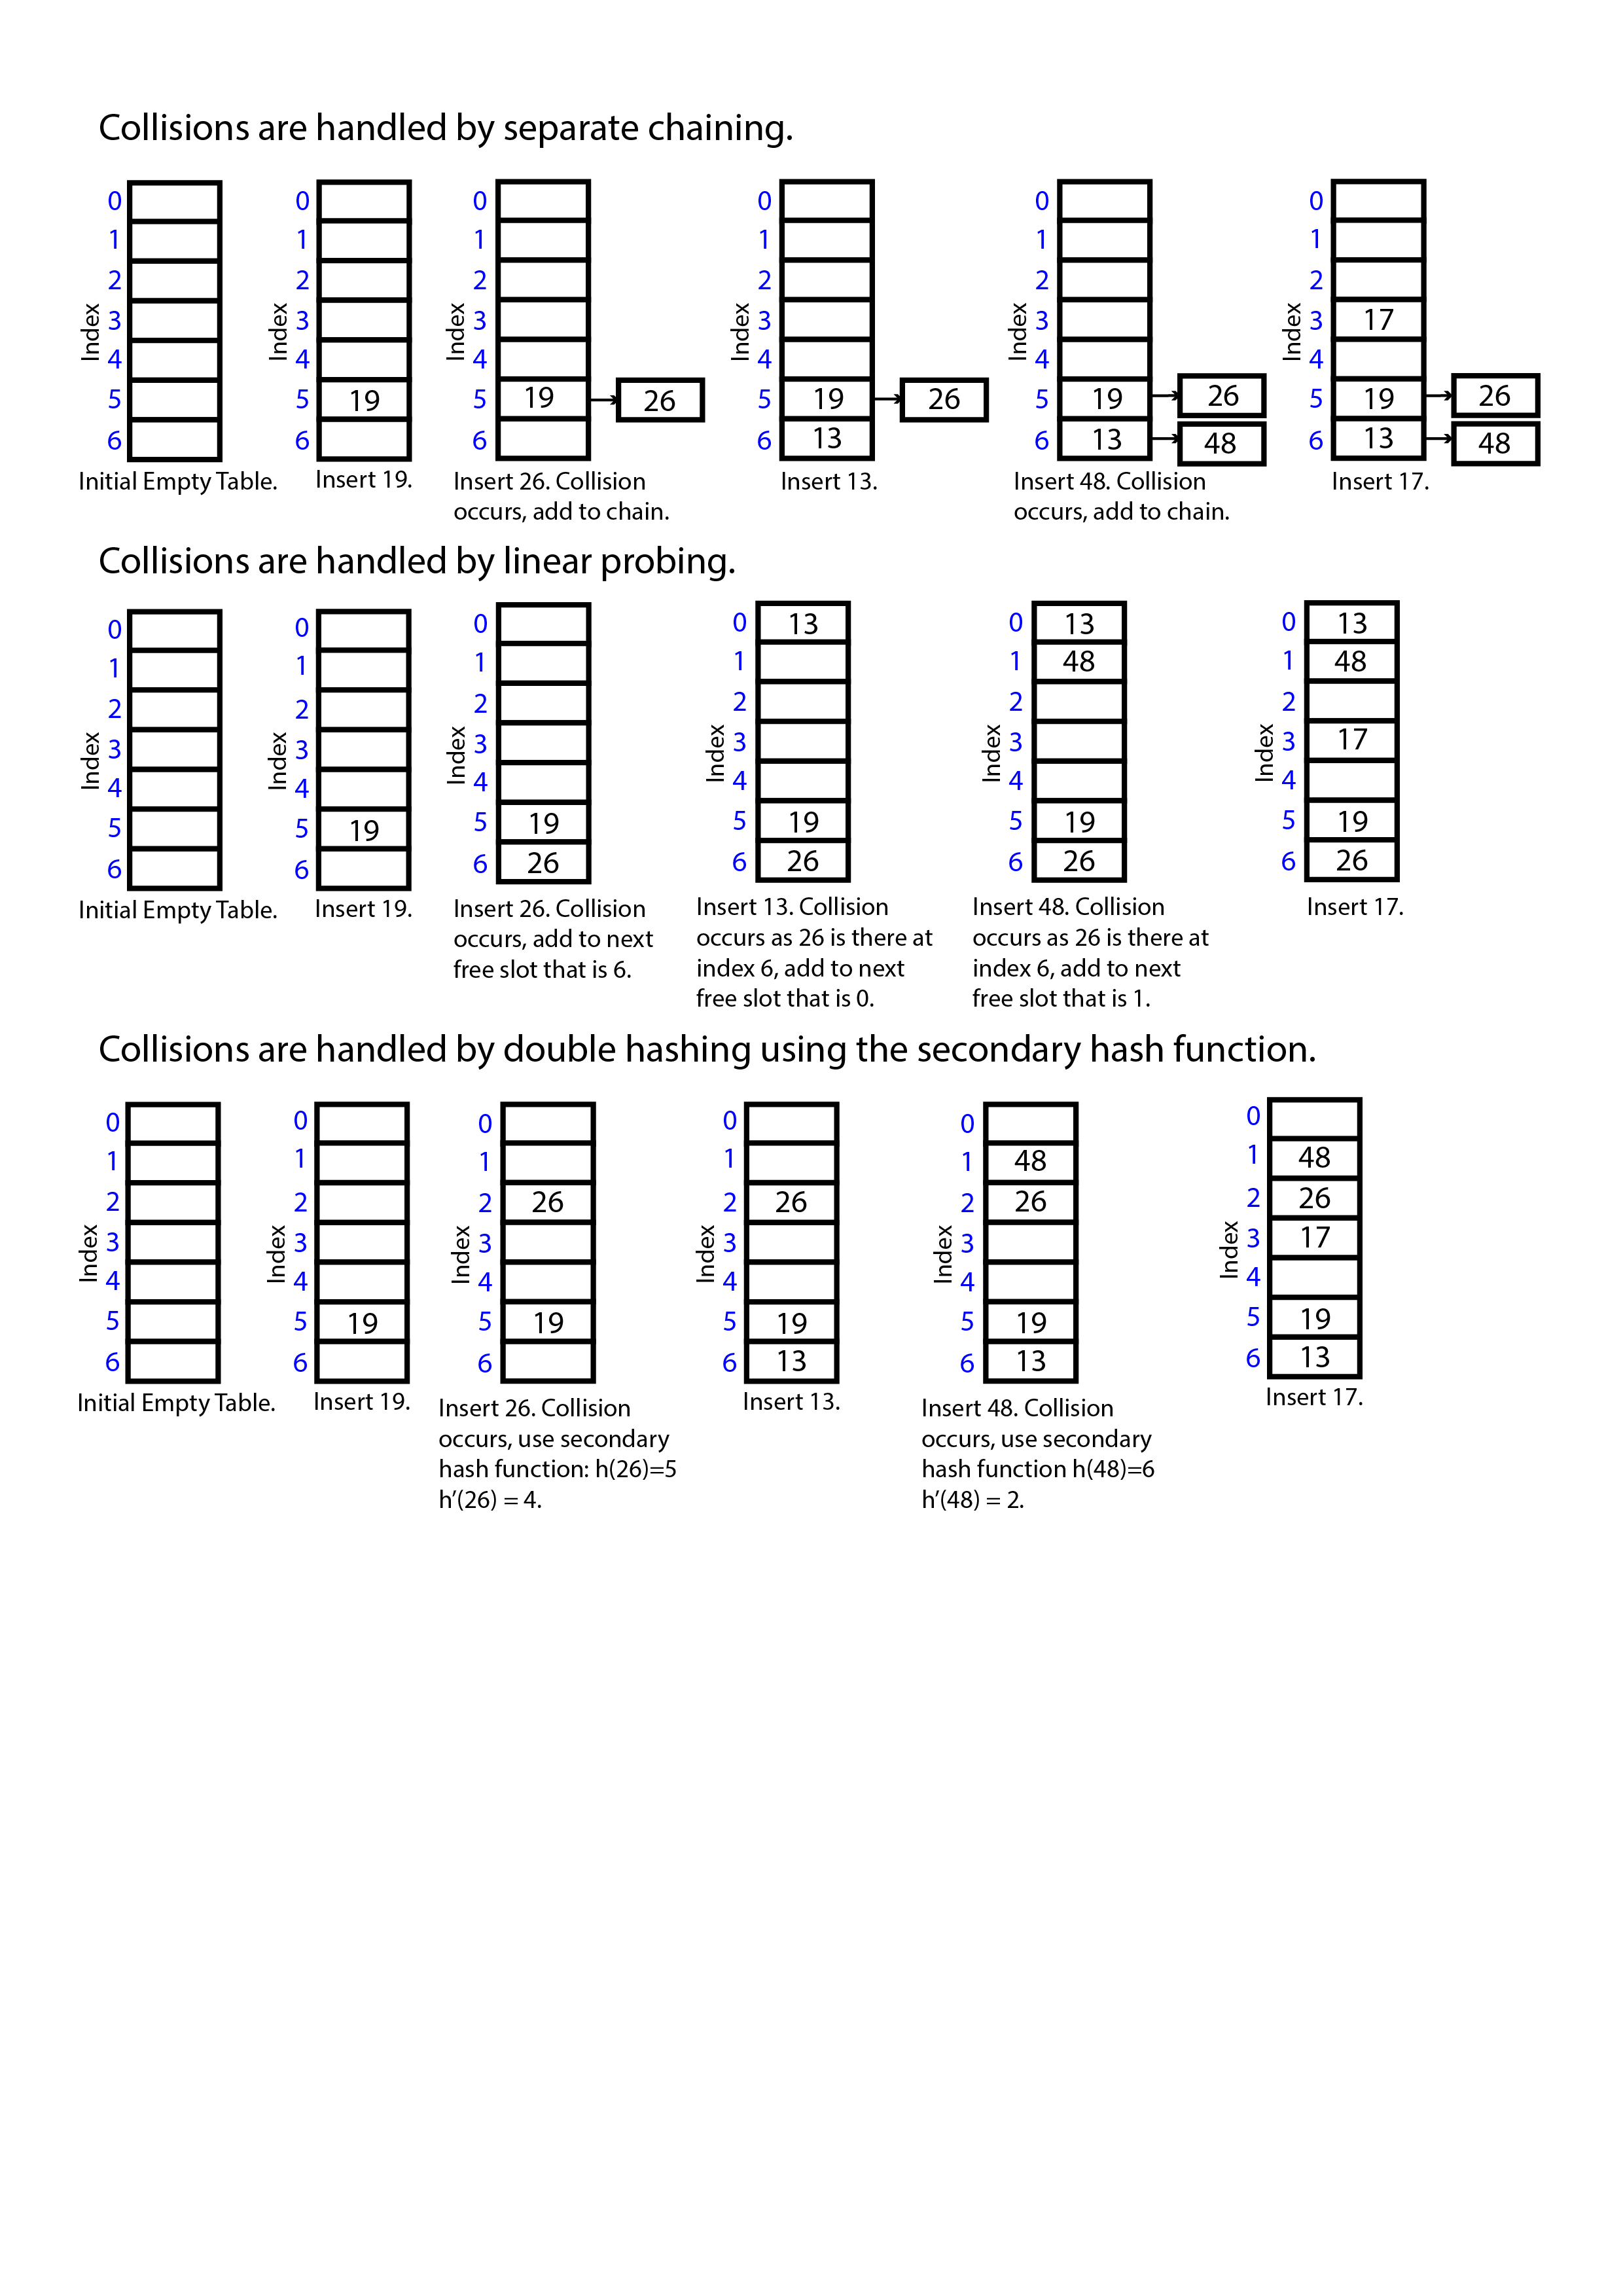
\includegraphics[width=0.8\linewidth]{Hashing.jpg}
\caption{Hashing}
\label{fig:mpr}
\end{figure}


\bigbreak
\noindent $\textbf{3.2. Hashing}$.\\
$h(x)=k$ \textbf(mod) $7$\\
The Figure 1 (page 3) shows tables with results after inserting for each of the scenarios below:\\
\noindent 1.When collisions are handled by \textbf{separate chaining}.\\
\noindent 2.When collisions are handled by \textbf{linear probing}.\\
\noindent 3.When collisions are handled by \textbf{double hashing} using the secondary
hash function $ h'(k)=5 - (k$ \textbf{mod} $5)$.\\

\noindent$\textbf{First scenario}$\\
Insert 19: $h(19)=5$. Add element to the 5th chain.\\
Insert 26: $h(26)=5$. Collision occurs, add element to the 5th chain (to the end of the chain or to the beginning depends on implementation, assume that this implementation implies inserting to the end of the chain).\\
Insert 13: $h(13)=6$. Add element to the 6th chain.\\
Insert 48: $h(48)=6$. Collision occurs, add element to the 6th chain.\\
Insert 17: $h(17)=3$. Add element to the 3rd chain.\\

\noindent$\textbf{Second scenario}$\\
Insert 19: $h(19)=5$. Put element to the slot 5.\\
Insert 26: $h(26)=5$. Collision occurs as 19 is there at index 5, put element to the next free slot that is 6.\\
Insert 13: $h(13)=6$. Collision occurs as 26 is there at index 6, put element to the next free slot that is 0.\\
Insert 48: $h(48)=6$. Collision occurs as 26 is there at index 6 and 13 at index 0, put element to the next free slot that is 1.\\
Insert 17: $h(17)=3$. Put element to the slot 3.\\

\noindent$\textbf{Third scenario}$\\
$H(k) =(h(k)+ih'(k))$ \textbf{mod} $7$\\
Insert 19: $h(19)=5$, $h'(19)=1$. Put element to the slot 5.\\
Insert 26: $h(26)=5$, $h'(26)=4$, $i=1$. Collision occurs, using secondary hash function. $H(k)=2$. So, put element to the slot 2.\\
Insert 13: $h(13)=6$, $h'(13)=2$. Put element to the slot 6.\\
Insert 48: $h(48)=6$, $h'(48)=2$, $i=1$. Collision occurs, using secondary hash function. $H(k)=1$. Put element to the slot 1.\\
Insert 17: $h(17)=3$, $h'(17)=3$. Put element to the slot 3.\\

\end{document}